\documentclass[conference]{IEEEtran}
\IEEEoverridecommandlockouts
\usepackage{cite}
\usepackage{amsmath,amssymb,amsfonts}
\usepackage{algorithmic}
\usepackage{graphicx}
\usepackage{textcomp}
\usepackage{listings}
\usepackage{xcolor}

\newcommand{\csh}{C{\#}}

\def\BibTeX{{\rm B\kern-.05em{\sc i\kern-.025em b}\kern-.08em
    T\kern-.1667em\lower.7ex\hbox{E}\kern-.125emX}}

\begin{document}

\title{Creating 3D games with Unity3D}

\author{\IEEEauthorblockN{1\textsuperscript{st} Boris Fuchs}
\IEEEauthorblockA{\textit{Mobile Computing} \\
\textit{University of Applied Sciences Upper Austria}\\
Hagenberg, Austria \\
boris.fuchs@students.fh-hagenberg.at}
\and
\IEEEauthorblockN{2\textsuperscript{nd} David Mitterlehner}
\IEEEauthorblockA{\textit{Mobile Computing} \\
\textit{University of Applied Sciences Upper Austria}\\
Hagenberg, Austria \\
david.mitterlehner@students.fh-hagenberg.at}
\and
\IEEEauthorblockN{3\textsuperscript{rd} Anika Seibezeder}
\IEEEauthorblockA{\textit{Mobile Computing} \\
\textit{University of Applied Sciences Upper Austria}\\
Hagenberg, Austria \\
anika.seibezeder@students.fh-hagenberg.at}
}

\maketitle

\begin{abstract}
\emph{The goal of this paper is to demonstrate the simplicity of Unity3D by creating a small 3D game. The focus is not only on scripting, but also on the features of the graphical editor provided by Unity3D.  To keep costs low, only freely available assets are used.}
\end{abstract}

\begin{IEEEkeywords}
Unity3D, 3D Games, 3D Environment, Character Controls, Animations
\end{IEEEkeywords}

\section{Introduction}
Nowadays creating realistic 3D games is getting a lot easier, due to various tools like Unity3D or the Unreal Engine. Game developers need little to no programming skills to make games in a minimum amount of time, because a great amount of premade assets and scripts are available for a very low cost. Most of the developing work can be done in the graphical editor, like creating 3D figures and adding properties, which can include self made scripts or physical properties. The majority of the existing game editors provide developing on multiple platforms including Smartphones and the most common game consoles. However Unity3D is better suited for devices with low end graphics cards, because it is more lightweight. Compared to the others, the available assets of Unity3D are not as high quality, but more economical on memory and graphics. \\ \\
The main point of this paper is: outlining the workflow of the game development process in Unity3D which consists of creating an environment and making a Third-Person-Character and some enemies.  \\
The first point of the game development process in Unity3D is to create an environment, with a small forest, some mountains and a few cottages. Then some textures are added to the components.
Secondly the Third-Person-Character is linked with a  script, so it can move around in the environment.
The third point is to create some enemies, that are chasing the player. 
Lastly animations for both, the character and the enemies, are provided and added to the game. \\ \\

\section{Creating an Environment (Written by Boris Fuchs)}

The following section focus at creating a simple environment with Unity3D. 
Unity3D provides an asset store, where all necessary assets (environment, scripts, characters,...) can be obtained. Anyone can offer his asset-packs in the store and other users can buy this asset-pack then. The prices of these asset-packs have a high variation, the range is from free usage to very expensive. 

\subsection{Preparing Unity3D}

For building a simple environment it is required to download the basic asset-pack of Unity3D and optional some other 3D-assets like trees or stones. This short environment demo is restricted to the Unity basic asset pack. The basic asset pack can be found in the store under \emph{Unity Essentials $\rightarrow$ Asset Packs $\rightarrow$ Standard Assets}.
After this step is finished, the assets can be involved in the current project or in that project where these assets be needed.

 
\subsection{Environment: First step}

Now its time to build a first terrain, the foundation of the prospective 3D-Models. A scale of 150 to 150 is an adequate base to represent the specified environment. As on fig.1 shown, the user can modify the scale at the last button in the terrain info template. All necessary (for this project) modifications can be done at the terrain info template. Take a look at the tabs that are interesting for crating a small environment. The first index tab is responsible for raise/lower the terrain. (e.g. for building mountains) The next two tabs can be ignored for this task. The fourth tab is for painting textures, and with the fifth tab (paint trees) the user is able to place trees at the terrain. The sixth tab is for painting details, more precisely for "painting" grass. With the last tab its possible to change the settings of the terrain, as before mentioned, to modify the scale. The next steps take a closer look at the various index tabs.
\begin{figure}[htbp]
  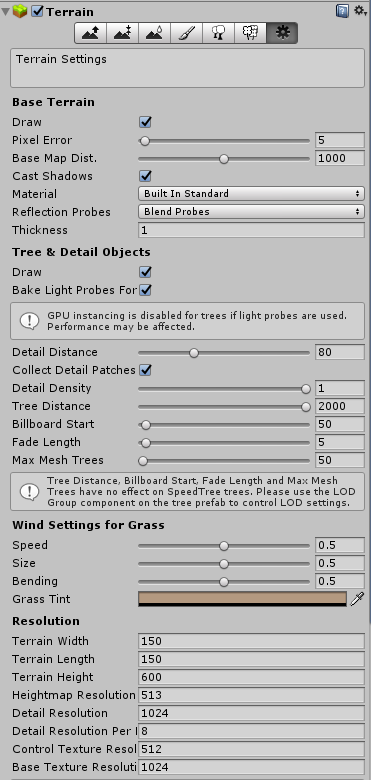
\includegraphics[width=.4\textwidth]{pictures/terrain_info}
  \caption{Terrain Info}
  \label{fig:terrain_info}
\end{figure}

\subsection{Environment: Raise/Lower Terrain}
This index tab has multiple brushes for lowering or raising the terrain. (see fig.2) The best way to find out which brush is the
best for altering the terrain, trying all brushes out and checking the effects will help. Additional there are settings for the brush where the user can change the brush size and the brush opacity. Depending on what the user wants to handle, these settings can be fit on every situation. To raise the terrain only click with the left mouse button and hold until the terrain is high enough. For lowering the user has to press and hold shift before clicking the left mouse button.
 
\begin{figure}[htbp]
  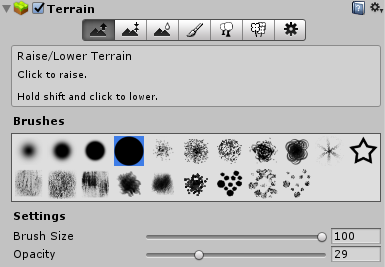
\includegraphics[width=.4\textwidth]{pictures/raise_lower_terrain}
  \caption{Raise/Lower Terrain}
  \label{fig:raise_lower_terrain}
\end{figure}

\subsection{Environment: Paint Textures}
One of the most important points is painting the textures. Without textures the most objects can not be identified. 
Like on the tab before here are also different brushes available for selection. The next step is creating a new texture. 
To choose between the different textures of the Unity3D standard asset pack, the user has to click on \emph{edit textures $\rightarrow$ add textures $\rightarrow$ select}. If everything worked, a view shows all available textures. The next two steps add the texture to the current project, first double click for adding the choose texture, then press add. Now the user can repeat this instructions for adding as much textures as want.

\begin{figure}[htbp]
  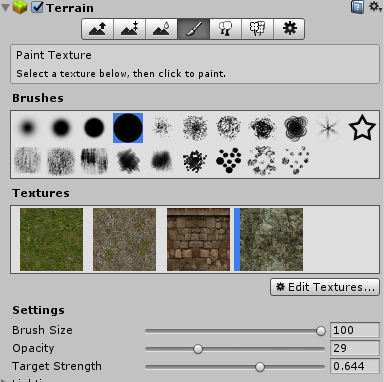
\includegraphics[width=.4\textwidth]{pictures/paint_textures}
  \caption{Paint Textures}
  \label{fig:paint_textures}
\end{figure}

\subsection{Environment: Paint Trees}
Inclose varying trees to project is nearly the same procedure as discussed in the chapter "Environment: Paint Textures". (\emph{edit trees $\rightarrow$ add trees $\rightarrow$ tree prefab $\rightarrow$ choose tree $\rightarrow$ double click $\rightarrow$ add})
Its possible to paint only one tree or to paint a lot of trees, depending on the brush size and the opacity. Now a lot of options are available. The key-features are: Adding other trees, mixing different trees and place it with a high brush size, place only a few trees or placing a dense forest depending on the current set opacity,....


\begin{figure}[htbp]
  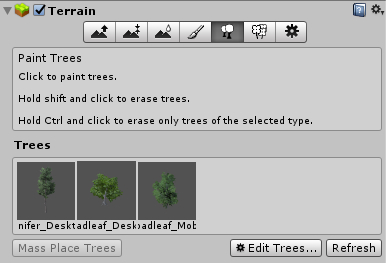
\includegraphics[width=.4\textwidth]{pictures/paint_trees}
  \caption{Paint Trees}
  \label{fig:paint_trees}
\end{figure}

\subsection{Environment: Paint Details}
The last section describes how to place grass on the terrain. The method to handle that is almost the same as before. Unity3D try’s to 
stay abreast of the same to guarantee a easy handling for users. The user has to click once again on (\emph{edit details $\rightarrow$ add grass texture $\rightarrow$ tree prefab}). After that, a small window appears where the user can change various settings. Inter alia it contains the minimum and maximum width and height plus settings to modify the color of the grass. (color can be change later, also when the grass is already placed) Selecting a grass is possible by clicking on detail texture and then double click on the decided grass texture like before. 


\begin{figure}[htbp]
  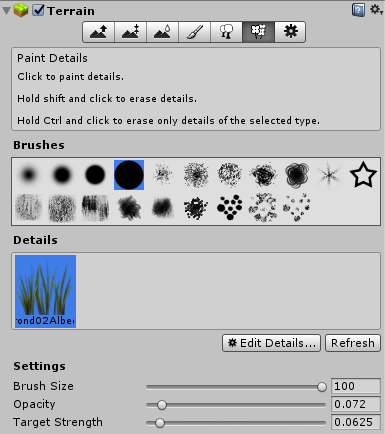
\includegraphics[width=.4\textwidth]{pictures/paint_details}
  \caption{Paint Details}
  \label{fig:paint_details}
\end{figure}

\subsection{Environment: Conclusion}
The user is now able to deal with the basic features of Unity3D creating an environment. But Unity3D provides much more features, settings and possibilities to create beautiful environment combined with an easy and clear handling. This short description illuminated only the recommended points to create a simple terrain with grass, trees and textures.


\section{Character Controls (Written by Anika Seibezeder)}

Character controls are a must have when developing a game. Otherwise the user would not be able to interact with a given character. No matter how hard the user is pressing a key or moving the mouse, the character still would not move at all.
With Unity3D the user interaction can be easily made by implementing scripts and adding them to the editor via Drag and Drop. The scripts can be written in \csh, JavaScript and Boo \cite{b1}. In the editor itself there is no opportunity to write the code, but there are several supported editors such as the recommended editor MonoDevelop by Unity3D or VisualStudio by Microsoft \cite{b1}.

\subsection{Adding a Character}

In Unity3D adding a character is easily done by dragging a Prefab or an object into the middle screen to the wanted position. There is also another possibility by dragging the Prefab or object to the left side of the screen, where all used objects are shown. A Prefab is a pre-built object combined of one to many components \cite{b2}. When downloading the Unity3D editor some prefabs are already given and can be used as is.
To see and edit features of the Prefab or object, a left click on the wanted object on the left side of the screen is needed. 

\begin{figure}[htbp]
  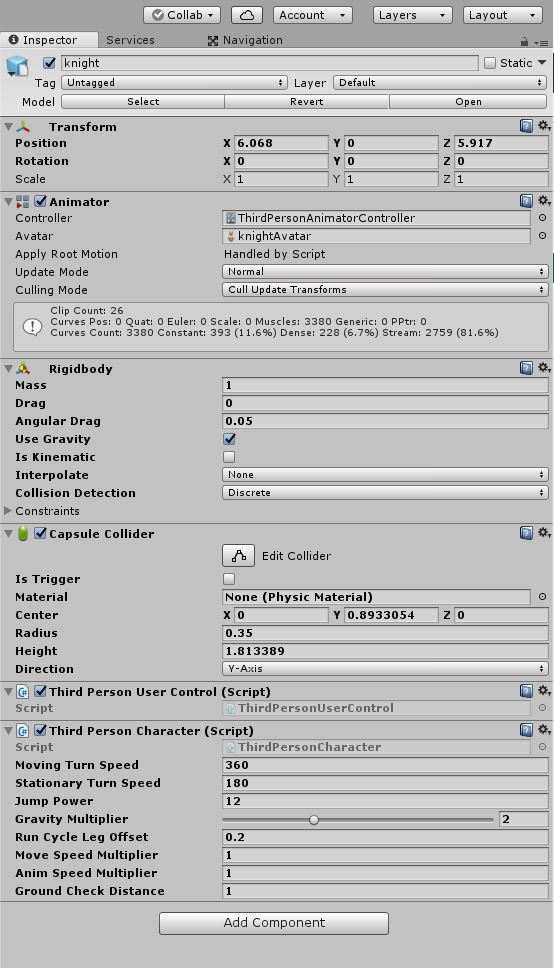
\includegraphics[width=.4\textwidth]{pictures/character_controls_character_components}
  \caption{Character Components}
  \label{fig:character_controls_character_components}
\end{figure}

As seen in figure~\ref{fig:character_controls_character_components}, a character has components like a Rigidbody, which gives the character a mass, a capsule collider, which triggers interrupts when colliding with other objects and scripts. Scripts can have some changeable variables like shown with the 2\textsuperscript{nd} script, or no changeable variable.

\lstloadlanguages{[Sharp]C}
\lstset{
basicstyle=\ttfamily\small,
numbers=left,
breaklines=true,
numberstyle=\tiny,
numbersep=5pt,
tabsize=3
}
\definecolor{listinggray}{gray}{0.95}
\definecolor{keyword}{rgb}{0.4, 0, 0.1}
\definecolor{comment}{rgb}{0, 0.4, 0}

\lstset{keywordstyle=\color{keyword}\bfseries}
\lstset{commentstyle=\color{comment}}
\lstset{backgroundcolor=\color{listinggray}}
\lstset{language=[Sharp]C}

\subsection{Scripting in VisualStudio}

A script is simply added by clicking the button "Add Component", choosing "New Script" and selecting the wanted language. After adding the script it can be written by double clicking the component and opening the wanted script editor. \\
The first thing to know about writing a script for Unity3D is, that the class is extending from the \lstinline!class MonoBehaviour! and is implementing the functions \lstinline!void Start()!, \lstinline!void Update()! and \lstinline!void FixedUpdate()!. 
The start function is used for variable initialization and one time execution.
The update function is used for continuous events, like checking which key is pressed, and is updated every frame\cite{b1}. As the user may press other keys while playing the game, the statements for checking the key should be implemented in the update function. Both functions are not necessarily needed but can help building the logic of the game.
Another important function is \lstinline!void FixedUpdate()!. Like the \lstinline!void Update()! function, it also is updated every frame and it is mainly used when dealing with the Physics of the Object \cite{b1}. \\
When adding variables there are just a few things to know: all \lstinline!public! variables are later shown in the component screen and can be edited there. It is also possible to import other components from the object. They are added to by using \lstinline!GetComponent<>()!

\subsection{Cross Platform Input Manager}

The Cross Platform Input Manager can be used to determine how keys or actions should be interpreted. For example there can be an entry considering jumping with a character, which defines, that a jump on a Desktop or Laptop is made with pressing the spacebar, while on the smartphone a touch gesture activates the jump. After defining the inputs, they can be used with \lstinline!CrossPlatformInputManager.GetButtonDown("Jump")!. \\

\begin{lstlisting}[caption=Example Implementation for Determining a Jump,label=list:character_controls_jump_implementation]
private bool isJumping;

private void Update()
{
	if (!isJumping)
	{
		isJumping = CrossPlatformInputManager.GetButtonDown("Jump");
	}
}
\end{lstlisting}

The code in Listing~\ref{list:character_controls_jump_implementation} shows how to implement the Cross Platform Input Manager in the \lstinline!void Update()! function which is updated every frame. 

\section{Adding Animations (Written by David Mitterlehner)}

The Unity editor supports various ways of adding animations to an object. The object can be simple, like a sphere, or complex, like a humanoid character with multiple joints. 

\subsection{Keyframes}

Animations can be implemented by setting keyframes in the "Animation" tab. Defining new keyframes is done by clicking the record button next to the media controls and moving the time cursor to the desired frame (e.g. frame 60). Any changes made to the object in the scene, for instance scaling or rotating, will now be recorded and saved to this keyframe (60). The transitioning frames between the keyframes are generated automatically by the editor. After setting the keyframe the animation can be previewed by clicking the play button in the media controls. In figure~\ref{fig:adding_animations_keyframes} there is one starting keyframe at position 0.
\begin{figure}[htbp]
  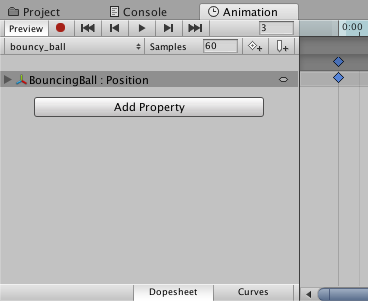
\includegraphics[width=.4\textwidth]{pictures/keyframes}
  \caption{Keyframes}
  \label{fig:adding_animations_keyframes}
\end{figure}

\subsection{State machines}

Multiple animations can be added to an object using state machines. State machines allow for complex transitions and event driven animations. The Unity editor provides a colored graphical overview for managing these transitions using semantics similar to state diagrams. Figure~\ref{fig:adding_animations_state_machines} shows the graphical overview of a simple state transition between to animations.
\begin{figure}[htbp]
  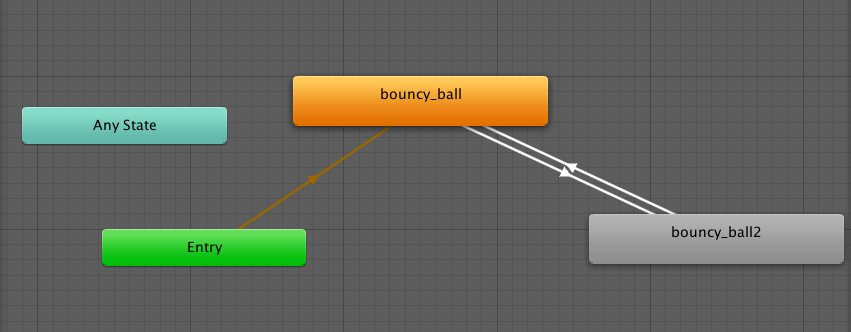
\includegraphics[width=.4\textwidth]{pictures/animation_states}
  \caption{Animation state machines}
  \label{fig:adding_animations_state_machines}
\end{figure}

\subsection{Basic animation concepts}

If keyframes are used for animating an object, say a bouncing ball, and no fine tuning of the duration of a single frame is performed, the animation isn't going to look very realistic. In 1981 Disney animators published a book called "The Illusion of Life", outlining the key concepts to making animations look realistic. In this publication, 12 concepts were defined, out of which two will be used here to illustrate how important fine tuning animations is for a natural look and feel of a 3D-game \cite{b3}.

\subsection{Timing}

The first, and arguably the most impactful concept covered here is timing. In the bouncing ball example, a linear progression of the frames doesn't look realistic, more frames need to be assigned to the top position (slow speed), and less to the bottom position (fast speed). In Unity this can be done by switching to the "Curves" tab on the bottom of the "Animation" tab, and editing the curve accordingly (See Figure ~\ref{fig:adding_animations_curves}). The steeper the slope, the faster the ball accelerates.

\begin{figure}[htbp]
  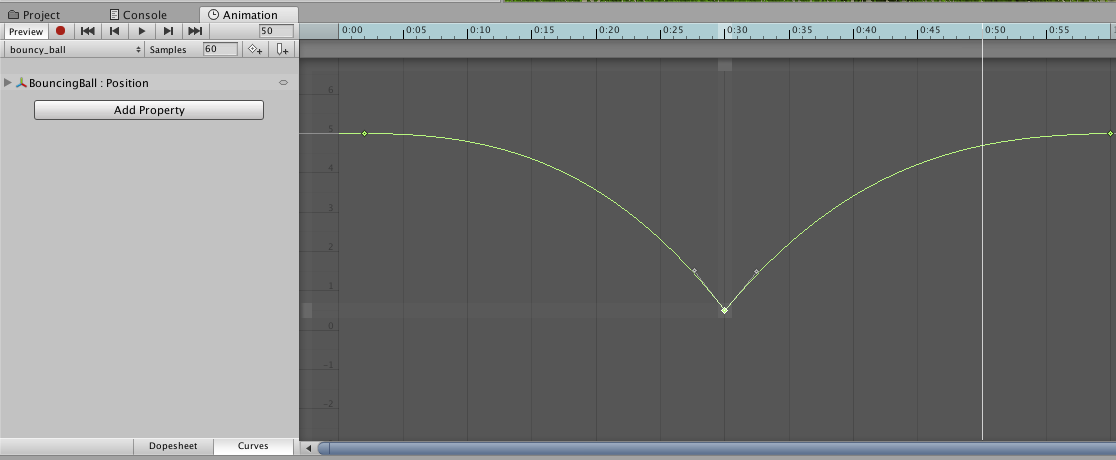
\includegraphics[width=.4\textwidth]{pictures/animation_curves}
  \caption{Animation curves}
  \label{fig:adding_animations_curves}
\end{figure}

\subsection{Squash and Stretch}

Another method for making an animated object look more realistic, is to transform the scale of the object as it moves, especially when it collides with another object. It is important that the volume of the object remains constant, however. In Unity this can easily be done by editing the X,Y, and Z scaling values of the object at a specific keyframe. Figure~\ref{fig:adding_animations_scaling} shows an example of this.

\begin{figure}[htbp]
  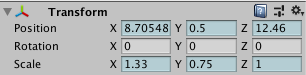
\includegraphics[width=.4\textwidth]{pictures/animation_scale}
  \caption{Editing the scale}
  \label{fig:adding_animations_scaling}
\end{figure}

\subsection{Complex character animations}

The bouncing ball is a trivial example, just to demonstrate the core concepts of animating in Unity. More complex animations, like character arm and leg movements, etc. can be obtained from the asset store. For example, there is a zombie asset on the store which includes walking, idle and attacking animations. An animator is also provided, which defines when, and under which conditions the animation states should be changed (Figure ~\ref{fig:adding_animations_zombie_states} and~\ref{fig:adding_animations_zombie_transition}).  To make the zombie actually walk towards the player and attack it, a script needs to be attached to it, for example the "AICharacterControl" script from the standard assets, where the player (knight) can be set as the target (See Figure~\ref{fig:adding_animations_zombie_script}).

\begin{figure}[htbp]
  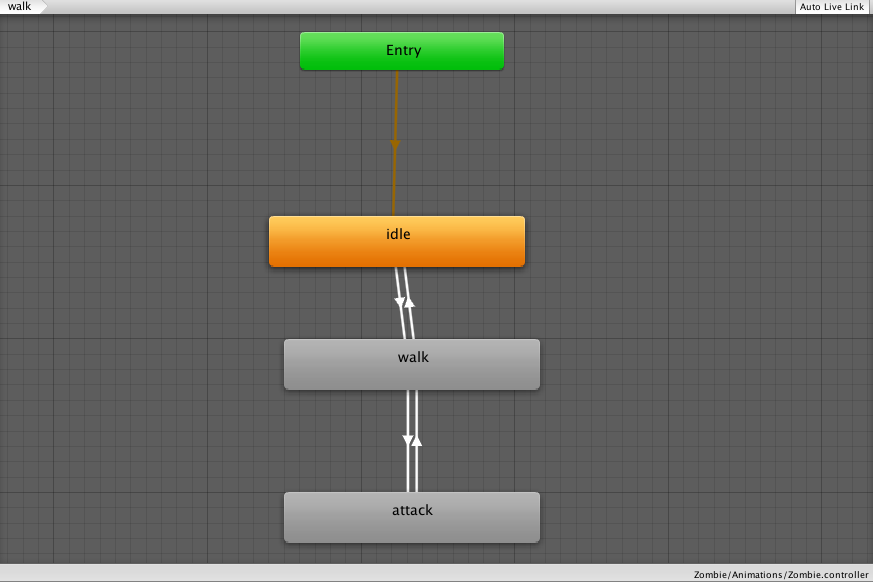
\includegraphics[width=.4\textwidth]{pictures/zombie_states}
  \caption{State diagram for the zombie character}
  \label{fig:adding_animations_zombie_states}
\end{figure}

\begin{figure}[htbp]
  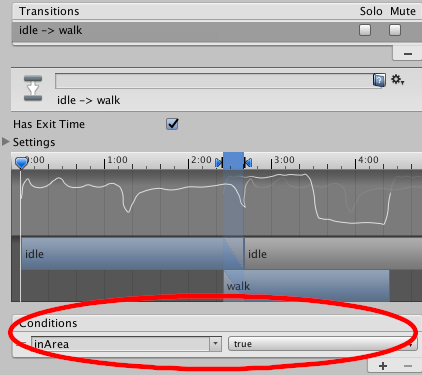
\includegraphics[width=.4\textwidth]{pictures/zombie_transition}
  \caption{Transitioning conditions for the zombie}
  \label{fig:adding_animations_zombie_transition}
\end{figure}

\begin{figure}[htbp]
  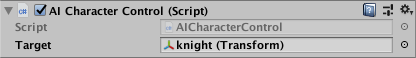
\includegraphics[width=.4\textwidth]{pictures/zombie_script}
  \caption{Script for the zombie}
  \label{fig:adding_animations_zombie_script}
\end{figure}

\section{Conclusion}

Unity3D provides an intuitive interface to assist the game designer throughout the entire workflow, from creating the terrain, to writing the scripts, to animating surrounding objects and the character. The asset store is one of the main features, since it frees the game designer from having to program every script themselves, or having to create 3D models from scratch. For advanced usage, everything can still be done manually, as has been shown in the "Character Controls" and "Adding Animations" sections. In conclusion, it can be said that Unity3D is a game design editor suitable for beginners, who need a lot of assistance and professionals, who want to build everything themselves.


\begin{thebibliography}{00}
\bibitem{b1} Ji Won Oak and Jae-Hwan Bae, "Development of Smart Multiplatform Game App using UNITY3D Engine for CPR Education", vol. 9, no. 7, pp. 263--268, 2014.
\bibitem{b2} Unity Technologies. "Manuel:Prefabs", Publication: 2018.1-002B, 2018.
\bibitem{b3} Thomas, Frank and Johnston, Ollie and Rawls, Walton, "Disney Animation: The Illusion of Life", 1981, Publisher: Abbeville Press New York
\end{thebibliography}

\end{document}
